\subsection{Kennzahlen}
    % TODO: Modell der Datenbank, um Labels etc. besser zu verstehen
    Anders als die Seite aus dem ersten Fallbeispiel wiederholt sich
    eine Nachrichtenseite nicht nur in mehreren Sites,
    sondern auch innerhalb einer Site.

    Die Klassifizierung wurde deshalb nicht auf allen Sites wiederholt,
    da keine neuen Erkentnisse zu erwarten sind.
    Ebenso wurden keine elementar anderen Ergebnisse für den Fall erwartet,
    alle Nachrichtenseiten in getrennten Datenbanken zu speichern.

    Mehr Potenzial für neue Ergebnisse scheint hingegen die Speicherung
    der Klassifikationen mehrerer Seiten eines Portals in einer Datenbank.
    Dieser Versuch wurde für das Portal "`B.A. Bildungswissenschaft"' durchgeführt,
    welches zu diesem Zeitpunkt fünf Nachrichtenübersischtsseiten enthielt.

    Die Aufteilung der Label auf die verschiedenen Knoten in in Tabelle
    \ref{table:findingsNewsFiguresNodesByLabel} zu sehen.
    Die Häufigkeit der Inhaltsklassen stellt Tabelle
    \ref{table:findingsNewsFiguresContentNodesByClass} dar.
    Tabelle \ref{table:findingNewsFiguresEdgesByLabel} zeigt die Aufteilung
    der Labels auf die Kanten der Datenbank und Tabelle
    \ref{table:findingsNewsFiguresEdgesByStartEndNodeLabel}
    stellt heraus, welche Knotenarten diese Kanten verbinden.
    Zuletzt betrachtet Tabelle \ref{table:findingsNewsFiguresSharedNodes}
    die Frage, welche Knoten mehrfach referenziert wurden.

    Zur besseren Verständnis der präsentierten Kennzahlen,
    veranschaulicht Abbildung
    \ref{image:findingNewsFiguresDbModel}
    wie der Graph der Klassifikation aufgebaut ist.
    Wegen der beschriebenen Überschneidung mit Fallbeispiel 1 im Kopfbereich,
    sind diese identischen Elemente nicht dargestellt.
    Verzichtet wird ebenso auf die Darstellung von Referenzen,
    da diese lediglich Kanten von den dargestellten Content Knoten
    zu Resource Knoten sind.
    Welche Content Klassen welche Referenzen besitzen können,
    ist zusammen mit dem Klassifikationsmodell ersichtlich.

    \begin{figure}[htb]
        \centering
        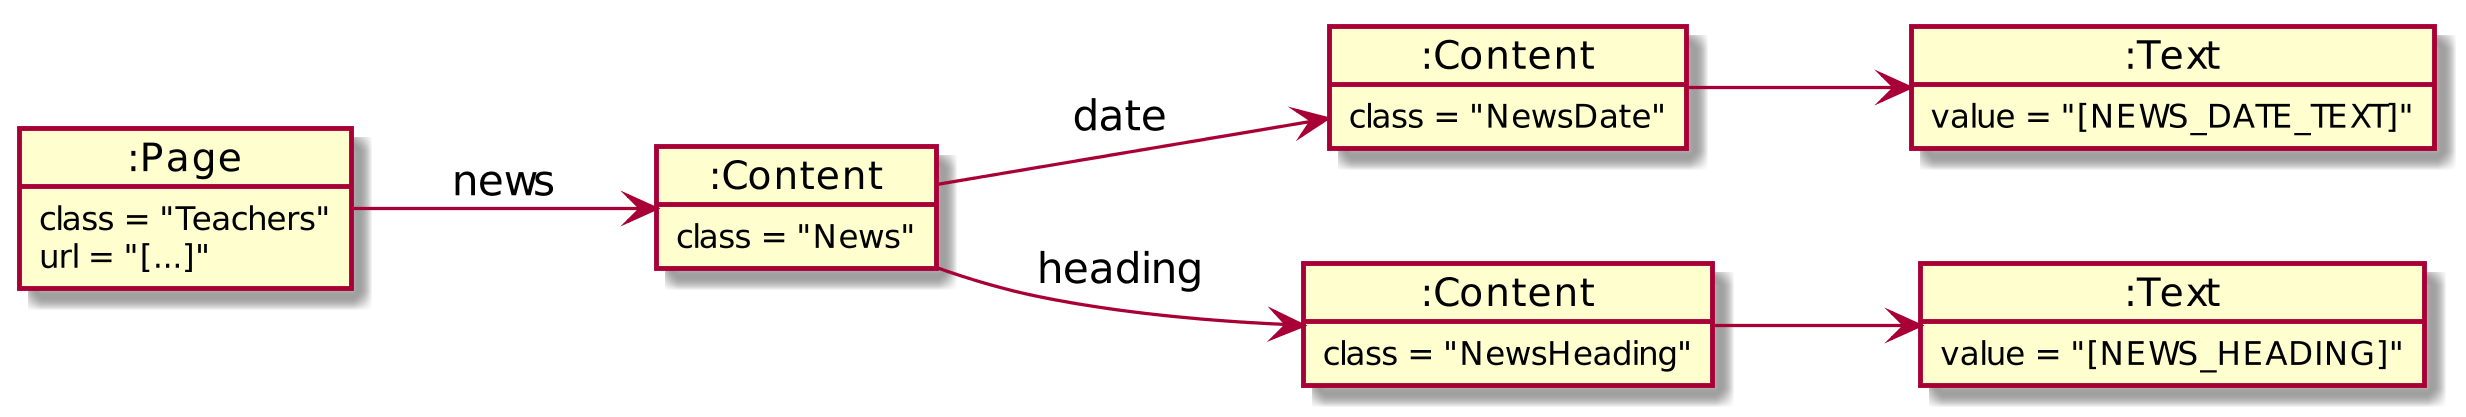
\includegraphics[width=\textwidth]{../resources/findings/case-study-2/dbmodel.png}
        \caption{Nachrichten DB Model}
        \label{image:findingNewsFiguresDbModel}
    \end{figure}

    Die Bedeutung einzelner Kennzahlen wurde bereits beim ersten Beispiel erläutert,
    die entsprechend auch hier gelten.

    \begin{table}[htb]
        \begin{subtable}[c]{0.3\textwidth}
            \centering
            \begin{tabular}{|l|c|}
                \hline
                \textbf{Label}  & \multicolumn{1}{l|}{\textbf{Anzahl}} \\ \hline
                Content         & 124                                  \\ \hline
                Page + Resource & 5                                    \\ \hline
                Resource        & 53                                   \\ \hline
                Site            & 1                                    \\ \hline
                Text            & 77                                   \\ \hline
                \hline
                \textbf{Summe}  & 260                                  \\ \hline
            \end{tabular}
            \subcaption{Anzahl der Knoten nach Label}
            \label{table:findingsNewsFiguresNodesByLabel}
        \end{subtable}
        \begin{subtable}[c]{0.3\textwidth}
            \centering
            \begin{tabular}{|l|c|}
                \hline
                \textbf{Klasse} & \multicolumn{1}{l|}{\textbf{Anzahl}} \\ \hline
                Brand           & 1                                    \\ \hline
                Header          & 1                                    \\ \hline
                News            & 41                                   \\ \hline
                NewsDate        & 38                                   \\ \hline
                NewsHeading     & 41                                   \\ \hline
                PageHeading     & 1                                    \\ \hline
                Portal          & 1                                    \\ \hline
                \hline
                \textbf{Summe}  & 260                                  \\ \hline
            \end{tabular}
            \subcaption{Content Knoten aufgeteilt nach Klassen}
            \label{table:findingsNewsFiguresContentNodesByClass}
        \end{subtable}
        \begin{subtable}[c]{0.3\textwidth}
            \centering
            \begin{tabular}{|l|c|}
                \hline
                \textbf{Label} & \multicolumn{1}{l|}{\textbf{Anzahl}} \\ \hline
                Reads          & 80                                   \\ \hline
                References     & 87                                   \\ \hline
                Owns           & 145                                  \\ \hline
                \hline
                \textbf{Summe} & 312                                  \\ \hline
                \end{tabular}
            \subcaption{Kanten nach Label}
            \label{table:findingNewsFiguresEdgesByLabel}
        \end{subtable}

        \begin{subtable}[c]{0.5\textwidth}
            \centering
            \begin{tabular}{|l|c|}
                \hline
                \textbf{Start $\rightarrow$ Ziel} & \multicolumn{1}{l|}{\textbf{Anzahl}} \\ \hline
                (:Content) $\rightarrow$ (:Content)     & 83                                   \\ \hline
                (:Content) $\rightarrow$ (:Resource)    & 49                                   \\ \hline
                (:Page) $\rightarrow$ (:Content)        & 57                                   \\ \hline
                (:Page) $\rightarrow$ (:Page)           & 13                                   \\ \hline
                (:Page) $\rightarrow$ (:Resource)       & 25                                   \\ \hline
                (:Site) $\rightarrow$ (:Page)           & 5                                    \\ \hline
                \textbf{Summe}                    & 232                                  \\ \hline
            \end{tabular}
            \subcaption{Kanten nach Start und Zielknoten}
            \label{table:findingsNewsFiguresEdgesByStartEndNodeLabel}
        \end{subtable}
        \begin{subtable}[c]{0.5\textwidth}
            \centering
            \begin{tabular}{|l|c|}
                \hline
                \textbf{Knoten} & \multicolumn{1}{l|}{\textbf{Anzahl}} \\ \hline
                PageHeading     & 1                                    \\ \hline
                Portal          & 1                                    \\ \hline
                Header          & 1                                    \\ \hline
                News            & 1                                    \\ \hline
                NewsDate        & 1                                    \\ \hline
                Seiten          & 4                                    \\ \hline
                Unterseiten     & 5                                    \\ \hline
                :Text           & 2                                    \\ \hline
                \textbf{Summe}  & 16                                   \\ \hline
                \end{tabular}
            \subcaption{Mehrfach referenzierte Knoten}
            \label{table:findingsNewsFiguresSharedNodes}
        \end{subtable}
        \label{table:findingsNewsFigures}
        \caption{Kennzahlen der Nachrichtenübersichtsseiten}
    \end{table}